\chapter{Automatic Scene Conversion} 
\label{sec:systemarch}
This chapter introduces our system and the scene conversion pipeline. We detail the scene import process, the intermediate state of the data and how we convert this information into the desired output renderer.

\section{System Architecture}
Our system is a Proof of Concept (PoC) that consists of two main components: an {\it import module} that reads an arbitrary scene file format and generates an equivalent description in a {\it canonical} scene representation; and an {\it export module} that takes our canonical representation and exports it to a target rendering system file format. The complete process is illustrated in Figure \ref{fig:sysarch}. 

Currently, our system supports \textit{PBRT v3}~\cite{PBRT:v3}, \textit{Mitsuba}~\cite{mitsuba}, and \textit{LuxRender}~\cite{luxrender}, as these are three of the most popular rendering systems. This architecture, however, is quite flexible. Supporting additional rendering systems only requires specializing the import and export methods to handle the new formats. Next, we describe the main components of our system.

\begin{figure}[h]
  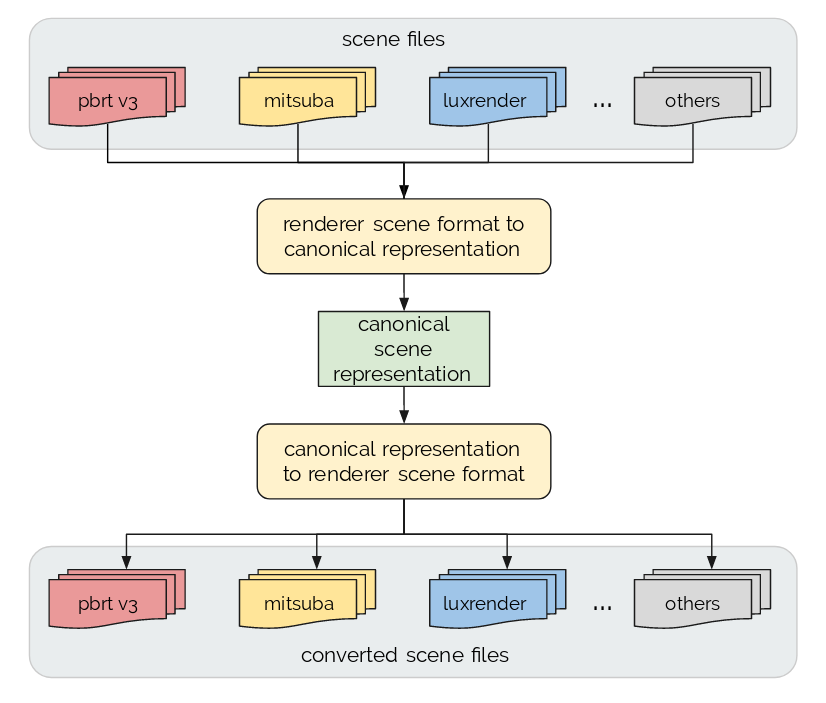
\includegraphics[width=\textwidth,height=\textheight,keepaspectratio]{images/4_system_architecture/architecture.png}
  \caption{Our scene conversion pipeline. An input scene description is imported into a canonical representation, which, in turn, can be exported to a target rendering system format.}
  \label{fig:sysarch}
\end{figure}

\section{The Import Module}
Most physically-based renderers subdivide the scene description in two main sections: {\it scene-wide rendering options} and {\it world block}. The former defines the rendering settings, while the latter describes the scene geometry and materials.

The import module parses the input scene files and translates each directive into a canonical representation. Since rendering systems use proprietary file format, both the import and export modules have to be specialized for each renderer.

PBRT and LuxRender scene descriptions consist of structured text statements. We generated parsers for these systems using PLY \cite{ply}, a Python implementation of Lex and Yacc.

Mitsuba, meanwhile, is a heavily optimized, plugin-oriented renderer. Its file format is, essentialy, an XML description of which plugins should be instantiated with the specified parameters. Since there are several XML-parsing libraries for Python, we chose to use ElementTree \cite{ET}, a Python XML parsing tool.

\section{Canonical Scene Representation}
While most renderers have a similar structure, they differ in a few supported features and in the parameters used to configure the rendering process. Thus, we need a canonical representation that covers the features supported by all renderers. 

COLLADA~\cite{collada} is an XML schema intended as a representation for exchanging digital content among graphics applications. However, COLLADA files only include information about the scene geometry. No information about other rendering options, such as camera positioning or integration techniques, is available. 

In order to establish a common ground for conversion, we defined a canonical scene representation. It is illustrated in Figure~\ref{fig:canonicalrep} and can easily extended to incorporate any directives not covered in our current implementation.
 
Our canonical representation mirrors the general structure of scene files and divides the scene data into scene-wide {\it rendering options} and {\it world block}. 

This is illustrated in Figure~\ref{fig:canonicalrep}, where the attributes stored for each scene component are shown on the rectangles on the right.

\begin{figure}[h]
  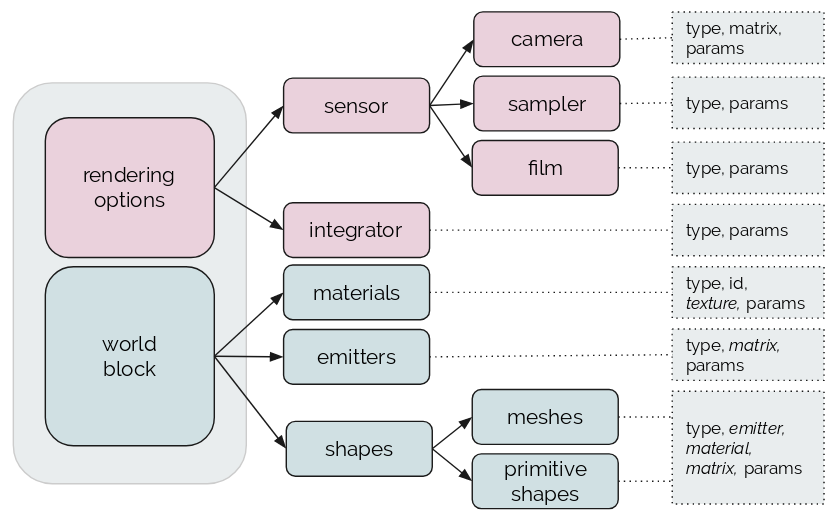
\includegraphics[width=\textwidth,height=\textheight,keepaspectratio]{images/4_system_architecture/canonicalrep.png}
  \caption{Structure of our canonical scene representation, consisting of rendering options and scene data. The attributes stored for each component are shown on the rectangles on the right.}
  \label{fig:canonicalrep}
\end{figure}

The \textit{Rendering Options} specify the integration and sampling techniques used for rendering, as well as camera and film properties. These include, for instance, camera position, camera matrix, image resolution, field of view, etc. Table~\ref{tab:summary} summarizes all types, parameters, and additional attributes associated with each component of our canonical scene representation. 

The \textit{World Block} describes the materials, global emitters, and shapes present in the scene.

A {\it material} (\eg, glass, plastic, metal, etc.) may have one or more associated textures. {\it Global emitters} represent all kinds of light sources, except area light sources, which are represented as shapes. These include conventional environment, spot, directional, and point light sources, as well more specific ones such as {\it sun} and {\it sky}.

A {\it shape} can be a polygonal mesh or a geometric primitive such as a rectangle, disk, cube, or sphere, for instance. 

\begin{center}
    \begin{tabular}{ l | l | l | l }
    \hline
    Directive 		& Type 				& Params 			& Others		\\ \hline
    integrator		& path tracer 			& max depth 			& -			\\
			& bidirectional path tracer 	& russian roulette depth	&			\\
			& metropolis light transport	& photon count			&			\\
			& photon mapping		& photon mapping lookup radius	&			\\
			& progressive photon mapping	& number of iterations		&			\\
			& direct lighting		& number of markov chains	&			\\ \hline
    sampler		& random			& samples per pixel		& -			\\
			& stratified			& scramble			&			\\
			& halton			&				&			\\
			& sobol				&				&			\\ \hline
    film		& ldr				& image width			& -			\\
			& hdr				& image height			&			\\
			&				& filter			&			\\
			&				& file extension (png, ...) 	&			\\ \hline
    camera		& perspective			& fov				& view matrix		\\
			& orthographic			& lens apperture		&			\\
			& environment			& focal distance		&			\\
			& realistic			& shutter open			&			\\
			&				& shutter close			&			\\
			&				& near clip			&			\\
			&				& far clip			&			\\ \hline
    materials		& metal				& kd				& texture (id, type, params)	\\ 
			& glass				& ks				&			\\
			& substrate/glossy		& transmittance			&			\\
			& matte/diffuse			& reflectance			&			\\
			& translucent			& roughness			&			\\
			& uber				& IOR				&			\\
			&				& eta				&			\\
			&				& k				&			\\
			& 				& id				&			\\
			& 				& ...				&			\\ \hline
    shapes		& mesh (ply/obj)		& filename			& model matrix		\\
			& cube				& center			& area emitter		\\
			& rectangle			& radius			& unnamed material	\\
			& sphere			& points			&			\\
			& disk				& normals			&			\\
			& trianglemesh			& uv mapping			&			\\
			& 				& ...				&			\\ \hline
    global emitters	& environment mapping		& radiance			& model matrix		\\
			& point				& filename			& 			\\
			& spot				& from (origin)			&			\\
			& sun				& to (direction)		&			\\
			& sky				& area (spot)			&			\\
			& directional			& ...				&			\\
			& distant			&				&			\\
    \end{tabular}
\end{center}
    

\section{The Export Module}

The export module is at the core of our system. While the import module deals with a single proprietary scene representation at a time, the export module has to map between materials and scene properties from two proprietary representations. 

In this case, there are several delicate cases to consider. Matrix transformations, native shapes, environment mapping coordinates and, mostly, materials are
some of the components that vary greatly between renderers. In several situations, there is no direct mapping between them. Still, our system should provide an output representation that, once rendered with the target system, best approximates the results obtained by the source rendering system with the input scene description. 

Achieving such results required extensive experimentation with parameters of the various systems. Next, we discuss a few relevant aspects one should consider.    
  
\subsection{Matrix Conversion}
There are several issues to consider when converting matrices between renderers. Do the two renderers use different coordinate systems (either left-handed or right-handed)? Do they represent matrices in the scene file using a direct representation or its inverse-transpose? How is the object-world transformation represented for shapes?

Mitsuba uses a right-hand coordinate system, while PBRT and LuxRender use a left-hand one. This means that, when converting between Mitsuba and the other
two, one has to mirror the x-axis of all camera matrix transformations. This is also the case for environment map positioning and object-world transformations. Moreover, Mitsuba's scene files contain a world-to-camera transformation matrix (\ie, view matrix), while PBRT and LuxRender scene files use the view matrix inverse transpose.

\subsection{Material Conversion}
Materials are the most delicate aspect of scene conversion. Materials have spectral and roughness properties that absolutely must be correctly mapped. 
However, most renderers have very different implementations for common subsurface scattering models (BSDFs), making it hard to predict the mapping between the parameters of two such implementations.

Mitsuba uses a more physics-oriented approach: a material can be diffuse, conductor, dielectric, plastic, translucent, or a bumpmap. It also has other types of materials, but those are not supported in the current implementation of our system. The material type in Mitsuba changes as the material contains any form of surface roughness, becoming a ``rough'' version of itself (for instance, a rough metal becomes a roughconductor). PBRT and LuxRender materials have roughness parameters, making it unnecessary to change the material's name.

To represent the material's reflectance, PBRT and Mitsuba use one index of refraction ($\eta$) and one absorption coefficient (\textit{k}) per color channel. 
LuxRender, however, uses a so-called ``{\it Fresnel texture}'', specifying a single value of $\eta$ and \textit{k} for all channels. Alternatively, LuxRender allows the specification of a single RGB color value for the material's reflectance. Therefore, correctly converting metal colors between LuxRender and PBRT or Mitsuba is not well defined, and is not supported in the current implementation of our system.

\subsection{Shape Conversion}
Shape directives can be split into two categories: {\it primitive shapes}, which can be used to specify primitives such as {\it rectangles, disks, cubes}, and {\it spheres}; and {\it 3D meshes}, which are stored in external files. 

Converting primitive shapes requires more attention than converting external 3D meshes. Mitsuba has directives for rectangle, disk, cube and sphere, while PBRT and LuxRender do not. 

Mitsuba's primitives are defined by some parameters (\eg, vertex positions, radius) which can be modified by a transformation (model) matrix. To reproduce these primitives in PBRT and LuxRender, an {\it internal triangle mesh} must be used. This is done by specifying the position, normal, and texture coordinates for each vertex in the mesh representing a given primitive. One should note that these internal meshes do not use the same representation as the 3D meshes stored in files.

Converting PBRT and LuxRender internal triangle meshes into Mitsuba primitive shapes is a more involving process. Since Mitsuba's primitives have predefined coordinates, converting vertices from PBRT or LuxRender internal meshes into these coordinates requires obtaining the transformation matrix that maps PBRT or LuxRender vertices to Mitsuba's predefined points. Our system takes care of this automatically.

Converting external 3D meshes is simple, as all rendering systems have directives for this purpose. PBRT, however, does not support Object File Wavefront 3D
(.obj) files. In this case, our system issues a warning, making the user aware of the need to convert .obj files off-line.

\subsection{Global Emitter Conversion}
Global emitters can be used to emulate environment lighting, such as the sun, the sky, or an environment map. Converting global emitters can be tricky, mainly
because different rendering systems do not implement the same algorithms and directives. For instance, Mitsuba and LuxRender implement {\it sun} and {\it sky} directives, while PBRT does not.

A sun directive can be simulated in PBRT using a distant light. A sky directive can be simulated using an environment map of a clear sky. While PBRT and LuxRender access environment maps using spherical coordinates, Mitsuba uses a latitude-longitude format. Thus, a conversion between the two representations is required. 
  
Converting a PBRT distant light into a sun directive for Mitsuba or LuxRender is straightforward. However, converting a PBRT environment map into a sky directive lends to an ambiguous situation, as the converter would require additional information to decide whether the environment map should be treated as a regular environment map, or as a sky directive. Our system solves this ambiguity by asking the user if the environment map should be converted to a sky
emitter.

Another sensitive point to consider is converting environment mapping indexation. PBRT and LuxRender access environment maps using spherical coordinates, 
($\theta$, $\phi$) expressed in cartesian coordinates, while Mitsuba uses a latitude-longitude format.   

A conversion between the two representations is required, which can be done by correctly aligning the axis of both coordinate systems. 

\begin{figure}[h]
  \centering
  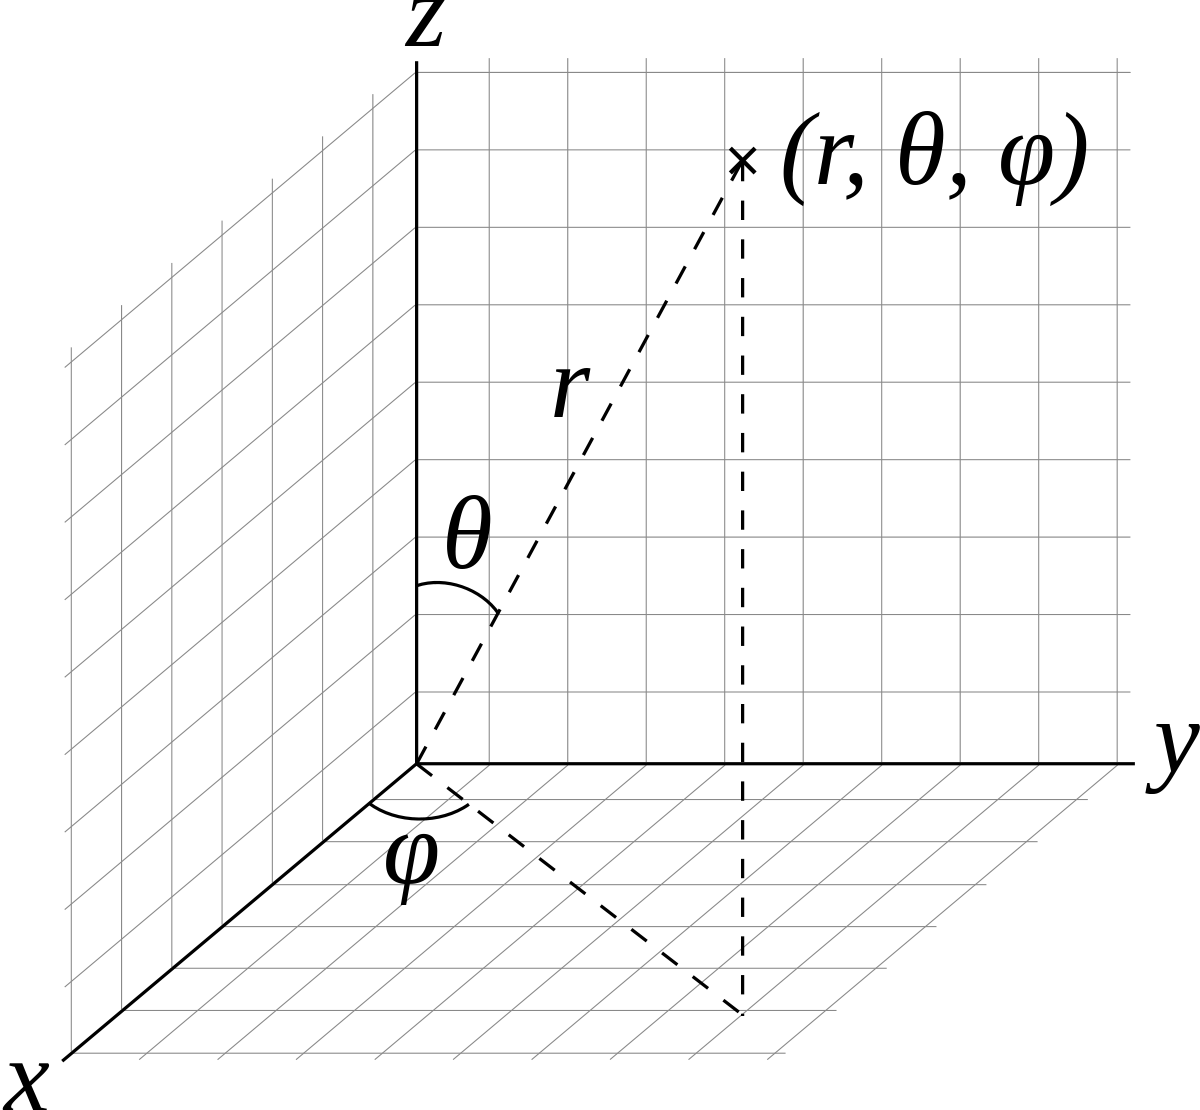
\includegraphics[width=0.7\textwidth,height=\textheight,keepaspectratio]{images/4_system_architecture/spherical_coordinates.png}
  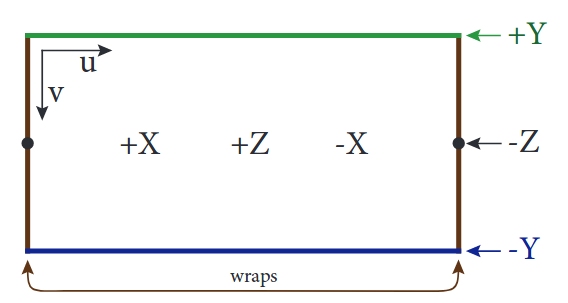
\includegraphics[width=0.7\textwidth,height=\textheight,keepaspectratio]{images/4_system_architecture/mitdocemitter.png}
  \caption{Illustration of the coordinate conventions used by PBRT and LuxRender 
  (top) and by Mitsuba (bottom) for indexing environment map uv coordinates.}
  \label{fig:mitdocemitter}
\end{figure}
